\documentclass[a4paper, 10pt]{article}
\usepackage{graphicx}
\usepackage[utf8]{vietnam}
\usepackage{indentfirst}
\usepackage{longtable}
\usepackage{fdsymbol}
\usepackage{color}
\usepackage{biblatex}
\usepackage{fullpage}
\usepackage{blindtext}
\usepackage{hyperref}
\usepackage{multicol}
\usepackage{caption}
\usepackage{amsmath}
\usepackage[table]{xcolor}
\usepackage{pgfplots}
\usepackage{subcaption}
\usepackage{tikz}

\addbibresource{main.bib}

\pgfplotsset{compat=1.16}

\hypersetup{
    pdftitle={XÂY DỰNG MÔ HÌNH SEQ2SEQ SINH CÂU TRUY VẤN SQL TỪ YÊU CẦU},
    hidelinks
}

\newtheorem{example}{Ví dụ}


\title{XÂY DỰNG MÔ HÌNH SEQ2SEQ SINH CÂU TRUY VẤN SQL TỪ YÊU CẦU}
\author{Kim Minh Thắng, Trần Gia Huy}
\date{Tháng 11 năm 2023}

% The preamble ends with the command \begin{document}
\begin{document} % All begin commands must be paired with an end command somewhere

\begin{titlepage}
    \begin{tikzpicture}[remember picture,overlay,inner sep=0,outer sep=0]
        \draw[blue!40!black,line width=4pt] ([xshift=-1.5cm,yshift=-2cm]current page.north east) coordinate (A)--([xshift=1.5cm,yshift=-2cm]current page.north west) coordinate(B)--([xshift=1.5cm,yshift=2cm]current page.south west) coordinate (C)--([xshift=-1.5cm,yshift=2cm]current page.south east) coordinate(D)--cycle;
    \end{tikzpicture}

    \begin{center}
        \fontsize{12pt}{17pt}
        \textbf{TRƯỜNG ĐẠI HỌC CẦN THƠ}

        \textbf{TRƯỜNG CÔNG NGHỆ THÔNG TIN VÀ TRUYỀN THÔNG}
    \end{center}

    \vspace{1cm}

    \begin{minipage}{\linewidth}
        \centering
        \includegraphics*[width=7cm]{logo-ctu.png}
    \end{minipage}

    \vspace{1cm}

    \begin{center}
        \fontsize{18pt}{17pt}
        \textbf{ĐỒ ÁN MÔN}
        \textbf{DEEP LEARNING - CT282 01}
    \end{center}

    \vspace{1cm}

    \fontsize{14pt}{17pt}
    \begin{center}
    \textit{\textbf{Đề Tài}}
    \end{center}

    \begin{center}
        \fontsize{16pt}{17pt}
        \textbf{XÂY DỰNG MÔ HÌNH SEQ2SEQ}

        \textbf{SINH CÂU TRUY VẤN SQL TỪ YÊU CẦU}
    \end{center}

    \vspace{1cm}

    \fontsize{14pt}{17pt}
    \textit{\textbf{Sinh viên thực hiện:}}

    \begin{tabbing}
        \hspace{6cm}\=\hspace{3cm}\=\kill
        {\it Trần Gia Huy}\>{\it B2016968 }\>\\
        {\it Kim Minh Thắng}\>{\it B2007210 }\>\\

    \end{tabbing}

    \vspace{2cm}

    \begin{center}
        {\it Cần Thơ, tháng 11 năm 2023}
    \end{center}
\end{titlepage}
\tableofcontents
\newpage

\listoffigures
\newpage

\maketitle % creates title using information in preamble (title, author, date)

\section{Giới thiệu}
\subsection{Bối cảnh đề tài}

\textbf{Ngôn ngữ truy vấn SQL} đã là một thành phần không thể thiếu của hệ quản trị cơ sở dữ liệu,
sử dụng trong gần như mọi hệ thống thông tin hiện tại. Việc sử dụng ngôn ngữ truy vấn SQL là một công việc hằng ngày của các lập trình viên.
Tuy nhiên, trong những câu lệnh SQL thường mang tính lặp lại, việc viết lại các câu lệnh này là một công việc tốn thời gian và công sức.

Những năm gần đây đã thể hiện sự phát triển mạnh mẽ của các mô hình \textbf{ngôn ngữ lớn (LLM)} - ứng dụng kiến trúc \textbf{Transformer} 
trong các bài toán xử lý ngôn ngữ tự nhiên (NLP).

\begin{minipage}{\linewidth}
    \captionsetup{type=figure}
    \centering
    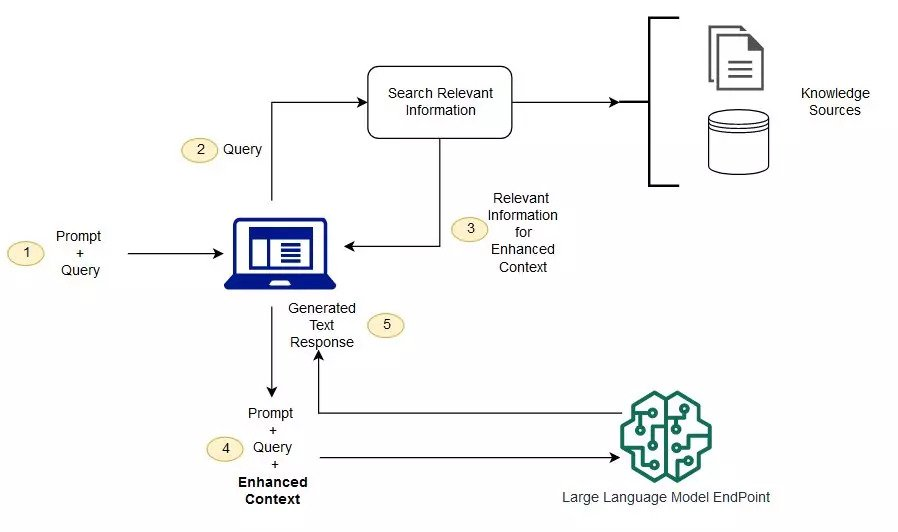
\includegraphics[width=14cm]{./llm.jpg}
    \caption{Quy trình hoạt động của các LLM. Nguồn ảnh: \textbf{Analytics Yogi}}
\end{minipage}

Ứng dụng lợi thế của các LLM, đồ án này đề xuất một mô hình \textbf{seq2seq} sử dụng kiến trúc \textbf{Transformer} để sinh câu truy vấn SQL từ yêu cầu người dùng.
Được fine-tune lại từ mô hình \textbf{T5} với 2 tập dữ liệu về câu hỏi với khoảng \textbf{310 nghìn} câu hỏi và truy vấn SQL tương ứng.

\newpage
\subsection{Đặt vấn đề}

Mục tiêu cuả đề tài chính là xây dựng một mô hình seq2seq sử dụng kiến trúc Transformer để sinh câu truy vấn SQL từ yêu cầu người dùng. Cụ thể hơn, mô hình cần sinh ra truy vấn SQL từ hai thông tin:
\begin{itemize}
    \item \textbf{Context}: Ngữ cảnh của câu truy vấn, ở đây chính là chi tiết về các bảng của cơ sở dữ liệu cần cho truy vấn. 
    
    VD: \textit{CREATE TABLE Customers (CustomerID int, CustomerName varchar(255));}
    \item \textbf{Question}: Câu hỏi tượng trưng cho câu truy vấn, được viết bằng Tiếng Anh.
    
    VD: \textit{What is the name of the customer with ID 1?}
\end{itemize}

Từ hai thông tin trên, mô hình cần sinh ra truy vấn SQL tương ứng:

\begin{itemize}
    \item \textbf{Answer}: Câu truy vấn SQL được sinh ra từ hai thông tin trên.
    
    VD: \textit{SELECT CustomerName FROM Customers WHERE CustomerID = 1;}
\end{itemize}

Mô hình cần đạt được một độ chính xác có thể chấp nhận được,
giúp giảm thiểu thời gian và công sức của lập trình viên trong việc viết các câu truy vấn SQL.

\subsection{Hướng tiếp cận}
Để giải quyết vấn đề này, hướng tiếp cận của đề tài chính là fine-tune lại mô hình transformer là \textbf{T5} - mô hình đưa tất cả bài toán về dạng text to text.

Fine-tune lại một mô hình ngôn ngữ lớn cần một lượng dữ liệu không nhỏ, sử dụng hai tập dữ liệu 
\textbf{b-mc2/sql-create-context} và \textbf{Clinton/Text-to-sql-v1} với tổng cộng khoảng 310 nghìn dòng dữ liệu.

\begin{minipage}{\linewidth}
    \captionsetup{type=figure}
    \centering
    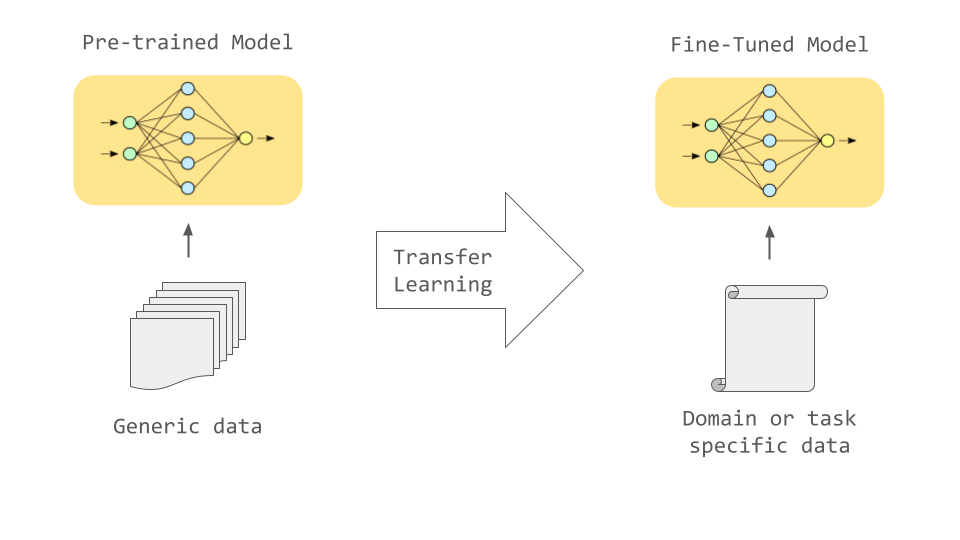
\includegraphics[width=14cm, height=10cm]{./finetune.png}
    \caption{Fine-tune LLM trên một downstream task. Nguồn ảnh: \textbf{Labellerr}}
\end{minipage}

\section{Tập dữ liệu fine-tune}
\subsection{Giới thiệu}
Cấu trúc chung của hai tập dữ liệu đều chứa 3 cột thể hiện:
\begin{itemize}
    \item \textbf{Ngữ cảnh câu hỏi}: Các câu lệnh CREATE TABLE để thể hiện những bảng dữ liệu cần dùng trong query.
    \item \textbf{Câu hỏi}: Câu hỏi tượng trưng cho câu truy vấn SQL, viết bằng Tiếng Anh.
    \item \textbf{Truy vấn SQL}: Câu truy vấn SQL được sinh ra từ hai thông tin trên.
\end{itemize}
Ngôn ngữ đươc sử dụng trong hai tập dữ liệu là Tiếng Anh, các câu lệnh SQL đều được viết đúng cú pháp, rất ít dữ liệu bị trùng lặp và bị thiếu. 

\subsection{Tập dữ liệu b-mc2/sql-create-context}
Tập dữ liệu bao gồm \textbf{78,577 dòng và 3 cột}
'question': ngôn ngữ tự nhiên cho câu hỏi, 'context' các câu lệnh CREATE TABLE,
'answer': Câu truy vấn SQL. 

Được xây dựng từ \textit{WikiSQL} và \textit{Spider}, mục tiêu của tập dữ liệu là dành cho các LLM text sang SQL. 
Sử dụng các lệnh CREATE TABLE để đưa ra ngữ cảnh cho câu lệnh rõ ràng hơn mà không cần đưa vào dữ liệu thật, tránh lộ thông tin riêng, giảm độ dài.

Chi tiết tập dữ liệu đọc thêm tại: \cite{b-mc2/sql-create-context}

\subsection{Tập dữ liệu Clinton/Text-to-sql-v1}

Tập dữ liệu bao gồm \textbf{262.000 dòng và 5 cột}

\begin{itemize}
    \item \textbf{instruction}: Câu hỏi để sinh ra truy vấn SQL.
    \item \textbf{input}: các câu lệnh CREATE TABLE.
    \item \textbf{response}: Câu truy vấn SQL đích.
    \item \textbf{source}: Nguồn của dòng dữ liệu.
    \item \textbf{text}: Diễn giải đầy đủ, kết hợp giữa cột instruction và input.
\end{itemize}


Chi tiết tập dữ liệu đọc thêm tại: \cite{Clinton/Text-to-sql-v1}

\section{Kiến trúc Transformer}
\subsection{Tổng Quan}

Transformer là một mô hình học sâu được giới thiệu bởi Vaswani và các cộng sự [9]
vào năm 2017, đây là mô hình đã đạt được kết quả nổi bật trong nhiều nhiệm vụ xử lý
ngôn ngữ tự nhiên (NLP). Transformer được xây dựng dựa trên cơ chế Attention
(Attention mechanism, tạm dịch: cơ chế tập trung), cho phép mô hình có khả năng “tập 
trung” vào các phần khác nhau của đầu vào (Input) trong quá trình học.

Mô hình Transformer sử dụng kiến thức đa đầu vào (Multi-Head Input) và đa đầu 
ra (Multi-Head Output) để xử lý đầu vào và đầu ra theo cách đồng thời, tức là không cần 
xử lý tuần tự từng phần như các mô hình trước đây. Điều này giúp giải quyết vấn đề độ
dài phụ thuộc trong ngôn ngữ (Long-range Dependency) và giúp mô hình có khả năng 
hiểu ngữ cảnh (Contextual Understanding) của dữ liệu đầu vào (Input).

Mô hình Transformer đã được ứng dụng rộng rãi trong nhiều tác vụ xử lý ngôn ngữ
tự nhiên, bao gồm dịch máy, phân loại văn bản, dự đoán từ, tóm tắt văn bản, hỏi đáp, và 
nhiều tác vụ ngôn ngữ tự nhiên khác. BERT (Bidirectional Encoder Representations from 
Transformers), GPT (Generative Pre-trained Transformer), và T5 (Text-to-Text Transfer 
Transformer) là những mô hình NLP nổi tiếng được xây dựng trên kiến thức của mô hình 
Transformer.

\begin{minipage}{\linewidth}
    \captionsetup{type=figure}
    \centering
    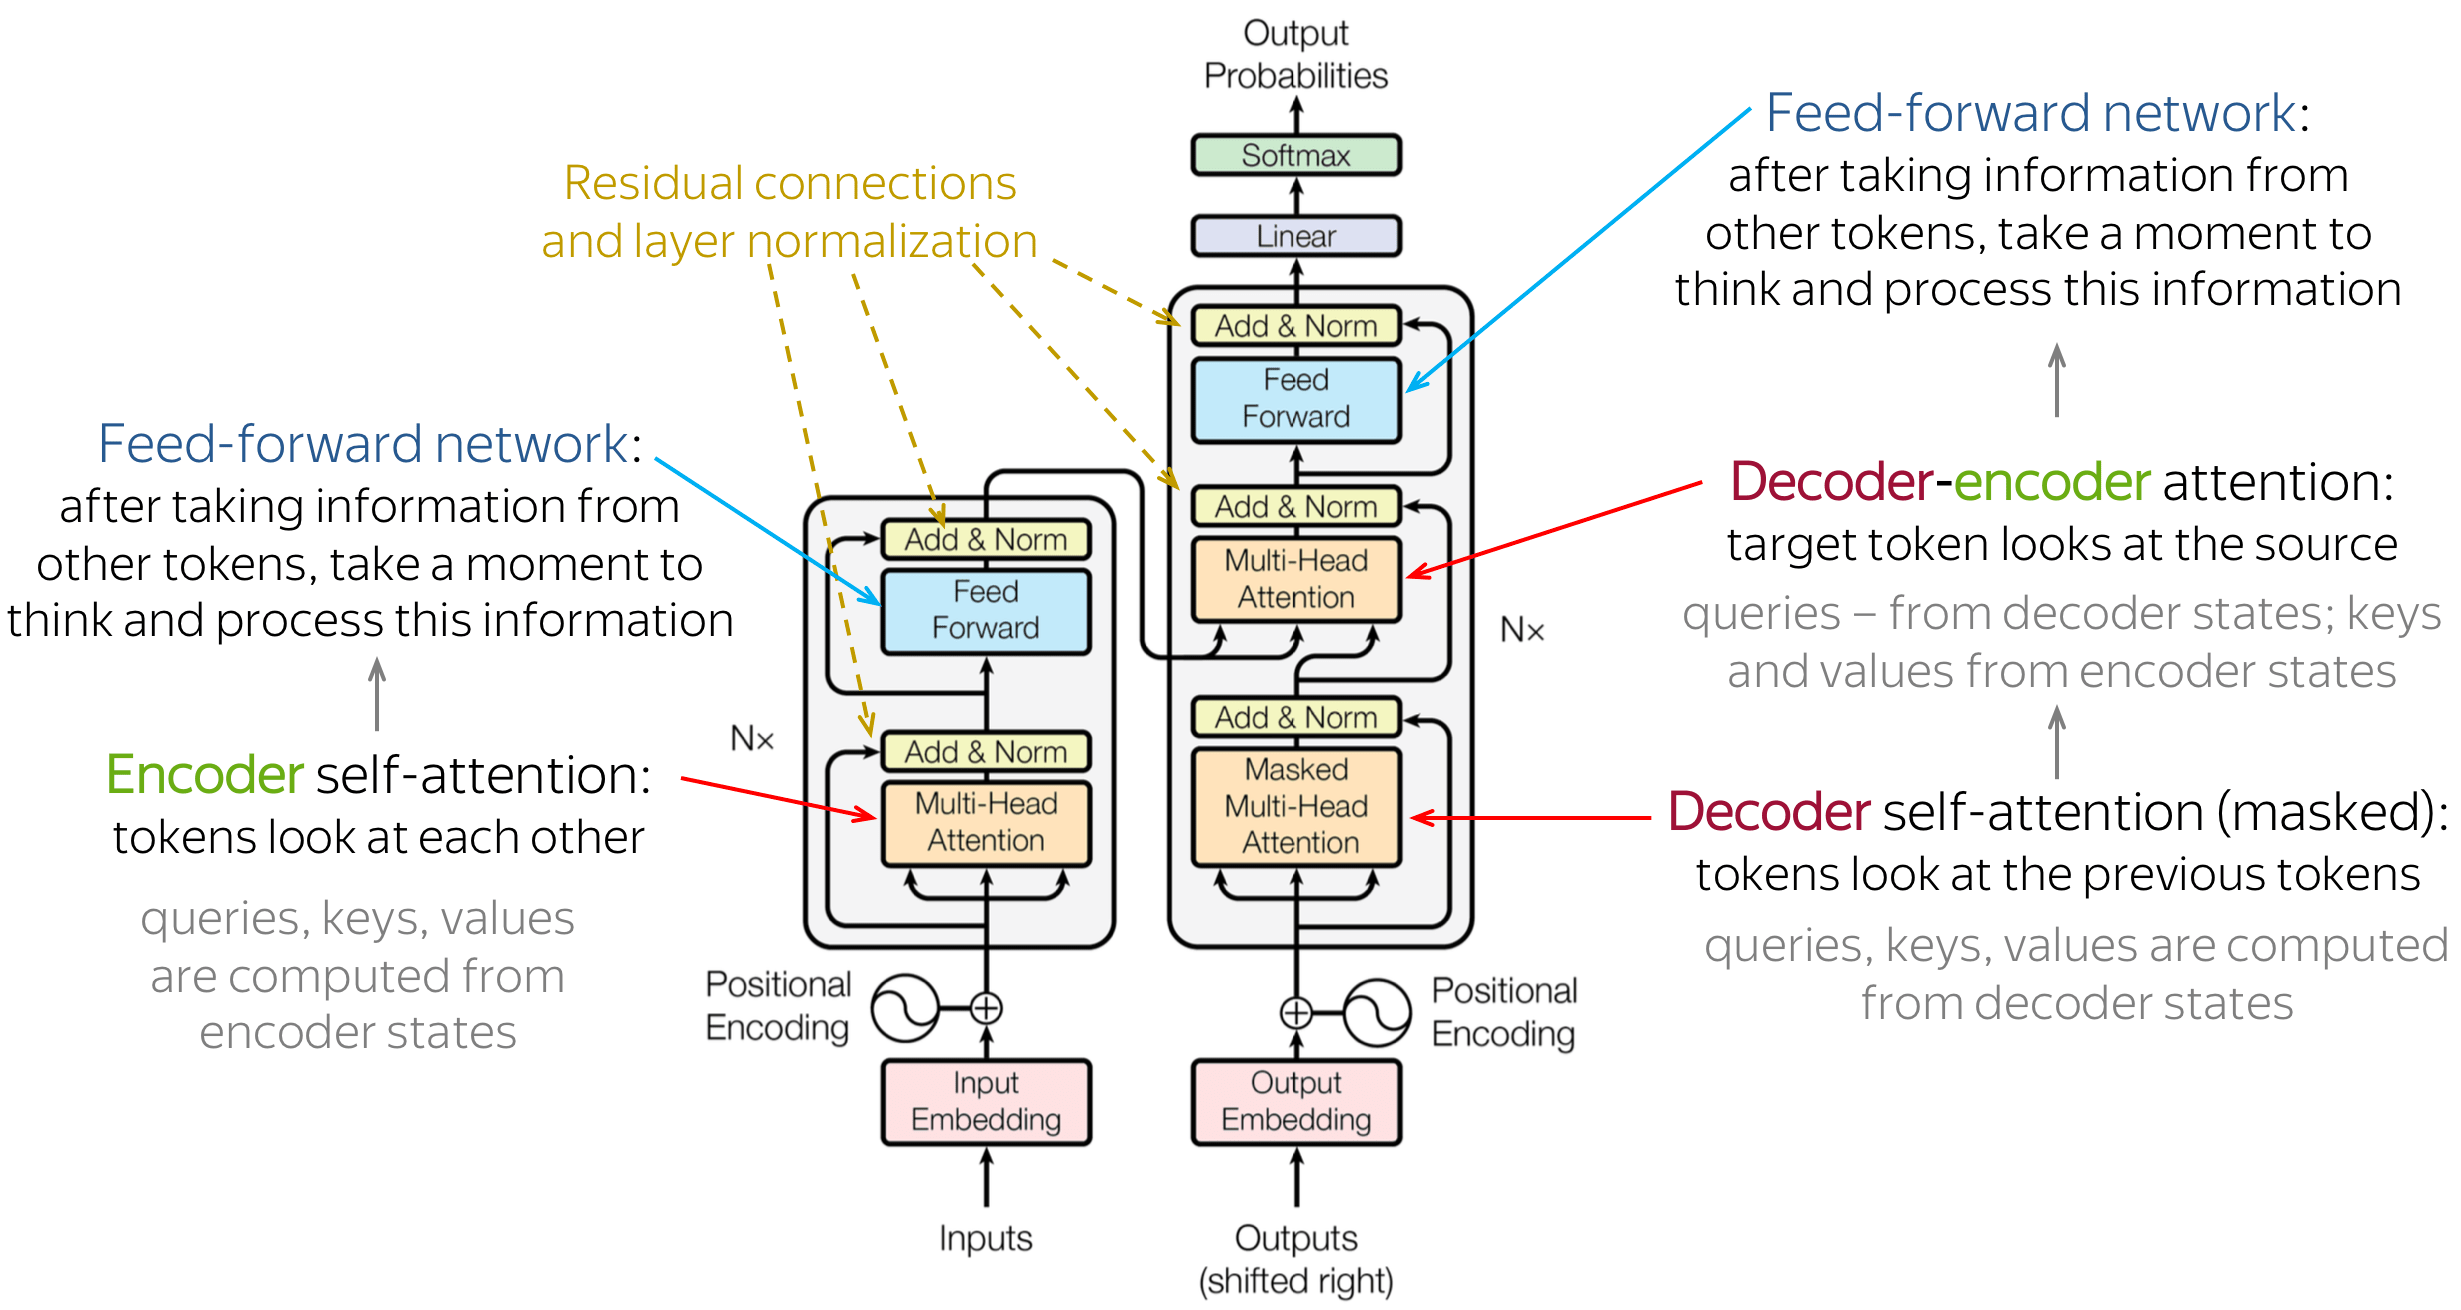
\includegraphics[width=14cm]{./transformer.png}
    \caption{Tổng quan kiến trúc Transformer. Nguồn ảnh: \textbf{Lena Voita}}
\end{minipage}

\begin{itemize}
    \item  Mô hình Transformer sử dụng định dạng mã hóa - giải mã (Encoder - Decoder) 
    tương tự như Seq2Seq.
    \item  Những khối được đề xuất trong Transformer, bao gồm Scaled Dot-Product 
    Attention và Multi-Head Attention, là trọng tâm của kiến trúc này, và chúng 
    được xếp hàng loạt và thực hiện song song (parallel) trong mô hình.
    \item Khác với kiến trúc của RNN,transformer, không có cấu trúc BPTT tương tự và tính toán 
    có thể được thực hiện song song, do đó mô hình có khả năng hoạt động hiệu quả
    hơn so với kiến trúc RNN.
\end{itemize}

\subsection{Hai khối Encoder và Decoder}
Đầu vào và đầu ra của Encoder có cùng kích thước. Do đó, cấu trúc Encoder có thể
được lặp lại nhiều lần để sử dụng một cách dễ dàng.

Tương tự, Decoder cũng có thể được lặp lại 
nhiều lần dưới dạng khối để giải mã đầu ra.

\begin{minipage}{\linewidth}
    \captionsetup{type=figure}
    \centering
    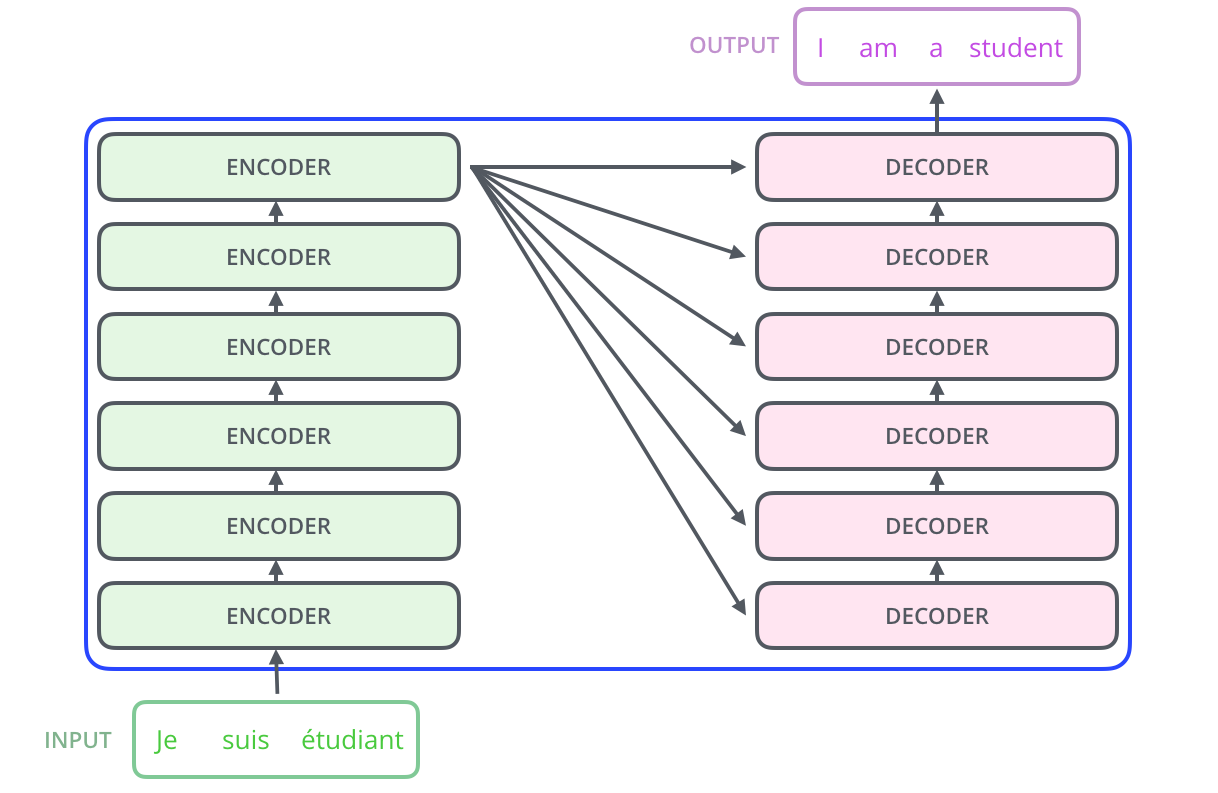
\includegraphics[width=10cm, height=5cm]{./The_transformer_encoder_decoder_stack.png}
    \caption{Chồng các khối Encoders và Decoders. Nguồn ảnh: \textbf{Jay Alammar}}
\end{minipage}

\subsection{Embedding và Positional Encoding}
\subsubsection {Input Embedding và Output Embedding}
Trong Transformer, Input Embedding và Output Embedding đều là tầng Embedding 
để chuyển đổi đầu vào thành vector với số thực.

Đây là tầng đầu tiên trong kiến trúc Transformer, nhận đầu vào là một 
one-hot-encoded vector là một vector có độ dài bằng với số từ trong từ điển,

Mỗi từ đi vào sẽ được tầng này tạo ra một vector đặc, có số chiều nhỏ hơn ban đầu.
\subsubsection {Positional Encoding}
Kết quả của tầng Input Embedding hoặc Output Embedding 
sẽ được đi qua một phép tính Positional Encoding.

\begin{minipage}{\linewidth}
    \captionsetup{type=figure}
    \centering
    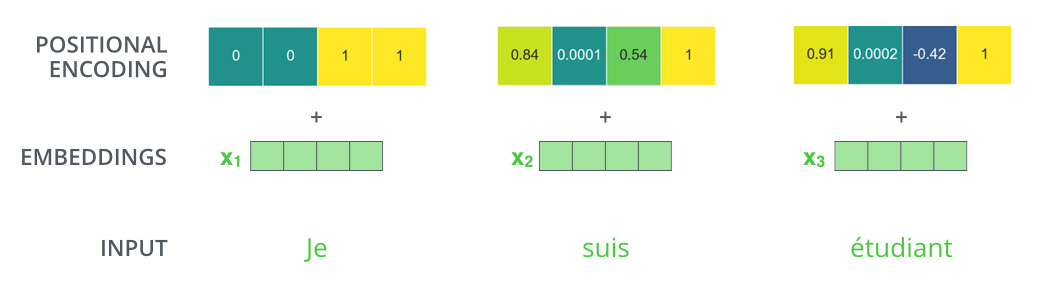
\includegraphics[width=14cm]{./transformer_input.png}
    \caption{Tầng Input và Output của Transformers. Nguồn ảnh: \textbf{Jalamar}}
\end{minipage}


Do Transformer không tính toán tuần tự mà xử lý một cách song song , nên nó không có khả năng 
nhận biết được vị trí của từ trong câu. Mục tiêu của phép tính
Positional Encoding là để giữ lại vị trí cho câu input, không làm mất thứ tự và ngữ nghĩa câu.

\subsection{Khối Multi-Headed Attention}
\subsubsection{Scaled Dot-Product Attention}
Attention là một cơ chế cho phép mô hình tập trung vào những phần quan trọng của đầu vào (Input) trong quá trình học. 
Cơ chế Attention được sử dụng trong nhiều mô hình NLP, bao gồm cả mô hình Transformer.

\begin{minipage}{\linewidth}
    \captionsetup{type=figure}
    \centering
    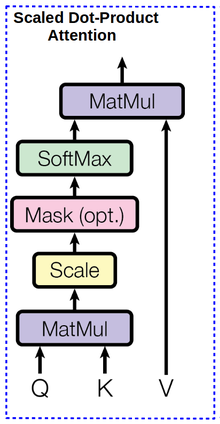
\includegraphics[width=6cm, height=8cm]{./ScaledDotProductAttention.png}
    \caption{Khối ScaleDotProductAttention. Nguồn ảnh: \textbf{PapersWithCode}}
\end{minipage}

Đầu vào của Scaled Dot-Product Attention là 3 ma trận Q, K, V có cùng số chiều.

Đầu ra của Scaled Dot-Product Attention là ma trận có cùng số hàng với ma trận Q và cùng số cột với ma trận V thể hiện trọng số attention của nó.

Dữ liệu trong khối này sẽ được xử lý như sau: \begin{itemize}
        \item Hai ma trận Q và K sẽ được nhân lại với nhau, sau đó chia cho căn bậc hai của số chiều 
        của ma trận K (tầng Scale) nhằm ngăn giá trị tăng lên quá lớn .
        \item Sau tầng Scale, nếu có tầng Mask thì sẽ được thực hiện để ngăn chặn Attention đến các kết nối không 
        hợp lệ (illegal connection).
        \item Sau đó, ma trận sau khi được nhân sẽ được đưa vào hàm softmax để chuẩn hóa giá trị Attention. Giúp mô hình tự tin hơn với các trọng số.
        \item Cuối cùng, ma trận sau khi được chuẩn hóa sẽ được nhân với ma trận V để tạo ra đầu ra của khối Scaled Dot-Product Attention. Đây chính là trọng số Attention của khối.
    \end{itemize} 

\subsubsection{Multi-headed Attention}

Thay vì chỉ sử dụng một khối Scaled Dot-Product Attention, Transformer sử dụng 
nhiều khối Scaled Dot-Product Attention song song (parallel) để tăng khả năng học của mô hình, hiểu ngữ nghĩa theo nhiều khối.

Đầu ra của mỗi khối Scaled Dot-Product Attention sẽ được nối với nhau và đi qua một tầng Linear để tạo ra đầu ra của khối Multi-Headed Attention.

Kết quả của khối là một ma trận có cùng số hàng với ma trận Q và cùng số cột với ma trận V thể hiện trọng số attention của nó.

\begin{minipage}{\linewidth}
    \captionsetup{type=figure}
    \centering
    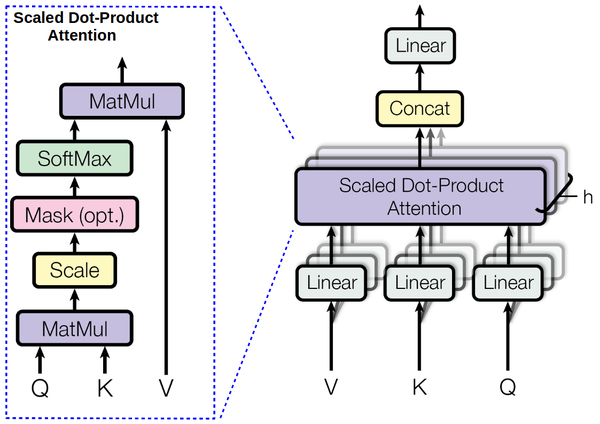
\includegraphics[width=6cm]{./MultiHead.png}
    \caption{Multi-headed Attention. Nguồn ảnh: \textbf{PapersWithCode}}
\end{minipage}

\subsection{Add và LayerNormalization}
Trong Transformer, Add \& Norm được sử dụng để kết hợp thông tin 
từ các tầng khác nhau trong mạng. Trong quá trình này, đầu ra của một tầng sẽ được 
cộng với đầu vào ban đầu của tầng đó (skip-connection), sau đó chuẩn hóa lại với Layer 
Normalization để tạo ra đầu ra cuối cùng. 

\begin{minipage}{\linewidth}
    \captionsetup{type=figure}
    \centering
    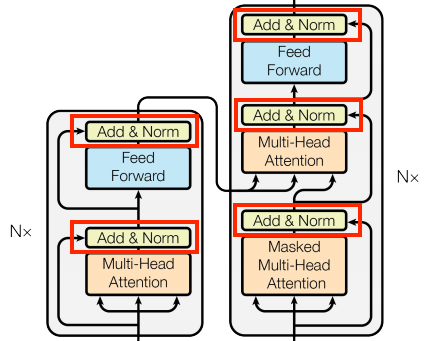
\includegraphics[width=6cm]{./Add+Norm.png}
    \caption{Tầng Add và LayerNormalization. Nguồn ảnh: \textbf{PyLessons}}
\end{minipage}
\subsubsection{Add}
Trong bước này, đầu ra của lớp sẽ được cộng với vector 
đầu vào ban đầu. Việc cộng này giúp cập nhật thông tin từ các phần khác nhau của kiến 
trúc và giúp tránh hiện tượng mất thông tin (Vanishing Gradient) trong quá trình huấn 
luyện.

\subsubsection{LayerNormalization}
Sau khi được cộng với đầu vào ban đầu, đầu ra của lớp sẽ được chuẩn hóa lại với
Layer Normalization. Layer Normalization là một phép chuẩn hóa dữ liệu đầu ra của
một tầng theo của ma trận đầu ra. Quá 
trình chuẩn hóa giúp cải thiện tính ổn định của mô hình 

\subsection{Position-wise Feed Forward Network}
\begin{minipage}{\linewidth}
    \captionsetup{type=figure}
    \centering
    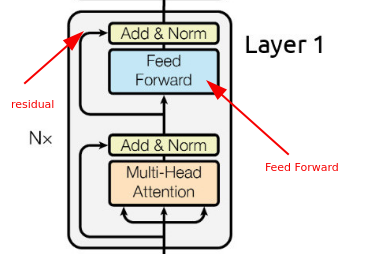
\includegraphics[width=6cm]{./feed-forward-sublayer-in-transformer.png}
    \caption{Khối Position-wise Feed Forward . Nguồn ảnh: \textbf{PyLessons}}
\end{minipage}

Các vector đầu vào (là các vector đại diện cho từ) sẽ được truyền qua tầng Fully Connected Layer với hàm kích hoạt ReLU, và cuối cùng đi qua một tầng Fully ConnectedLayer nữa.
Đầu ra của tầng thứ hai cũng chính ra đầu ra của Position-wise Feed-Forward. 

Mục đích chính là xử lý tiếp attention output từ tầng trước đó, giúp mô hình có thể học được các mối quan hệ giữa các từ trong câu.


\section{Mô hình T5 Small}
\begin{minipage}{\linewidth}
    \captionsetup{type=figure}
    \centering
    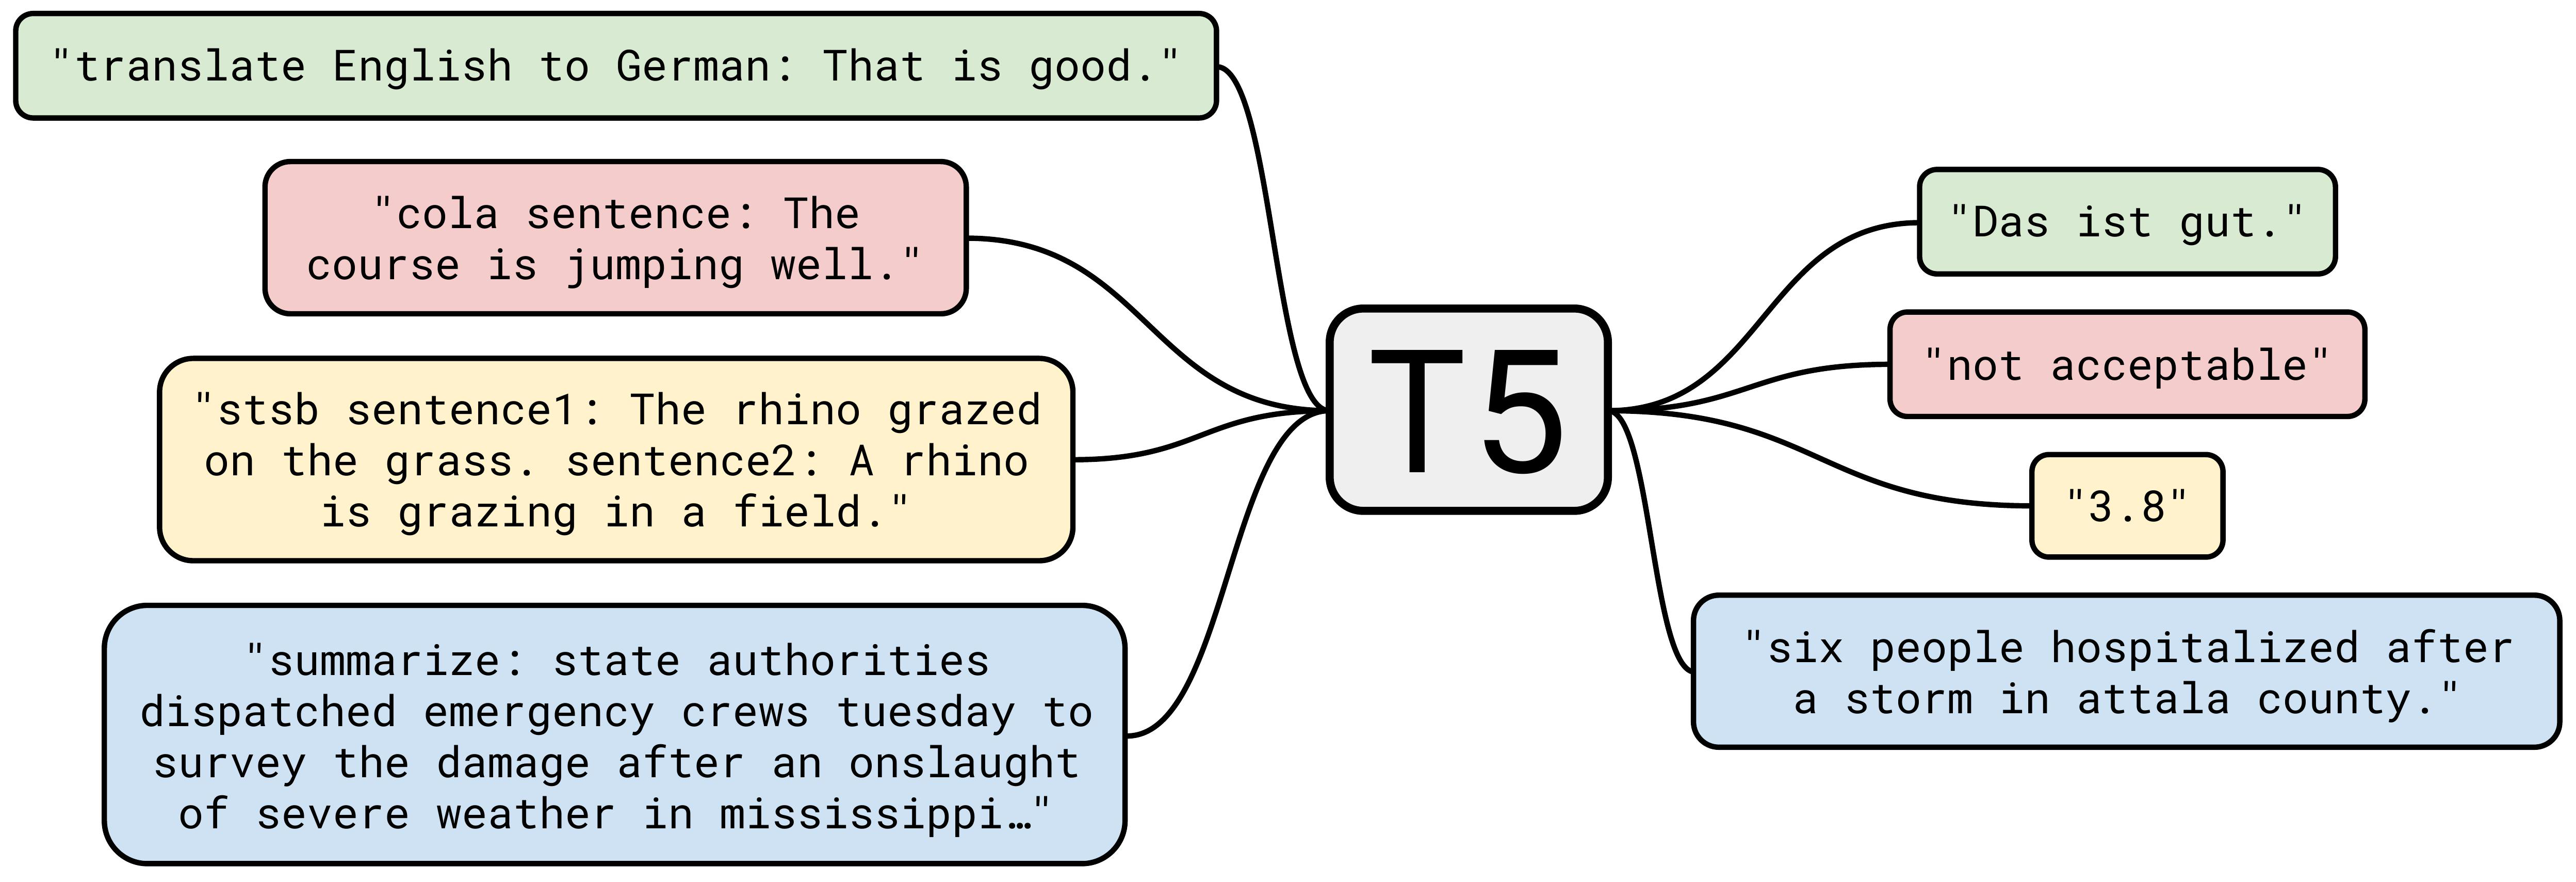
\includegraphics[width=14cm]{./t5.jpg}
    \caption{Mô hình T5 trong bài toán Text to Text . Nguồn ảnh: \textbf{Exploring the Limits of Transfer Learning with a Unified Text-to-Text Transformer}}
\end{minipage}

\vspace{0.5cm}
\subsection{Giới thiệu}
\textbf{Mô hình T5, hay Text-To-Text Transfer Transformer}, là một kiến trúc transformer nổi tiếng trong lĩnh vực xử lý ngôn ngữ tự nhiên (NLP). Mô hình này được giới thiệu 
bởi Google Research và ra mắt lần đầu tiên trong bài báo 
"Exploring the Limits of Transfer Learning with a Unified Text-to-Text Transformer" vào năm 2019.

Mục tiêu chính của T5 là đơn giản hóa các nhiệm vụ xử lý ngôn ngữ tự nhiên thành một định dạng chung gọi là \textbf{"text-to-text"}. Điều này có nghĩa là mô hình được huấn luyện để xử lý mọi công việc NLP thông qua việc chuyển đổi từ đầu vào thành đầu ra dưới dạng văn bản. Điều này bao gồm cả các nhiệm vụ như dịch máy, 
tóm tắt văn bản, phân loại văn bản, và nhiều nhiệm vụ khác.

Được huấn luyện bằng phương pháp \textbf{teacher-forcing} trên một lượng lớn dữ liệu, trong đó có tập dữ liệu C4 - một tập dữ liệu lớn được thu thập ở các trang web trên Internet. 
Mô hình được huấn luyện trên nhiều tác vụ khác nhau, nhờ vậy, có khả năng đáp ứng cho transfer learning.

\subsection{Pre-training T5}
Việc pre-training của mô hình T5 được thực hiện với cả  \textbf{Self-supervised Learning} và \textbf{Supervised Learning}.
\begin{itemize}
    \item Với \textbf{Self-supervised Learning}, mô hình được huấn luyện bằng cách sử dụng các \textbf{Corrupted Token}. 
    
    Bằng cách ngẫu nhiên xóa bỏ 15\% các token
    và thay chúng thành các "sentinel" token, ta sẽ tạo được các câu bị chỉnh sửa.
    Những câu bị chỉnh sửa sẽ là input cho khối encoder, câu gốc sẽ là input cho khối decoder, và các token bị bỏ ra giới hạn bởi các "sentinel token" sẽ là nhãn
    
    \begin{minipage}{\linewidth}
        \captionsetup{type=figure}
        \centering
        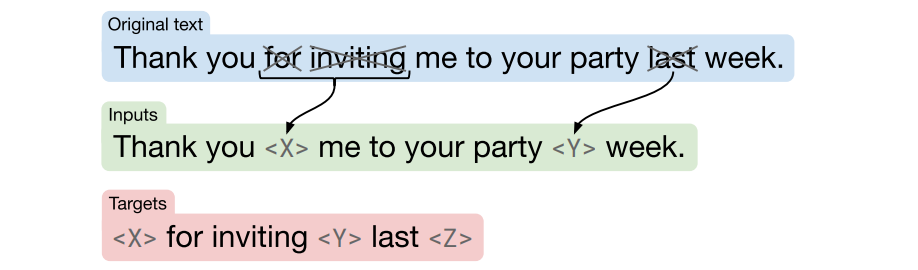
\includegraphics[width=14cm]{./t5_train.png}
        \caption{Self-supervised Training với T5 . Nguồn ảnh: \textbf{Exploring the Limits of Transfer Learning with a Unified Text-to-Text Transformer}}
    \end{minipage}

    \item Với \textbf{Supervised Learning}, mô hình được huấn luyện trên các tác vụ downstream được cung cấp bởi chuẩn GLUE và SuperGLUE (được đưa về dạng text to text).
\end{itemize}

\subsection{Tham số}
Với mô hình \textbf{T5 Small}, kiến trúc của nó sẽ dựa trên Transformer với:
\begin{itemize}
    \item 6 khối encoders và 6 khối decoders 
    \item 8 headed-attention
    \item Chiều dài của feed-forward layer là 2048
    \item Chiều vector đầu ra là 512
    \item Số lượng tham số là khoảng 60 triệu tham số.
\end{itemize}

\section{Fine-tune mô hình sinh truy vấn SQL từ yêu cầu}
Để có được mô hình sinh truy vấn SQL từ chuỗi câu hỏi và chuỗi ngữ cảnh, mục tiêu đề tài là fine-tune lại \textbf{mô hình T5} 
với hai dataset \textbf{sql-create-context} (78 nghìn dòng) và \textbf{Text-to-sql-v1} (262 nghìn dòng)


\subsection{Tiền xử lý dữ liệu}
Đầu tiên, dữ liệu được load từ huggingface datasets, sau đó được tiền xử lý theo các bước sau:
\begin{itemize}
    \item Loại bỏ các dòng dữ liệu bị thiếu.
    \item Loại bỏ các dòng dữ liệu bị trùng lặp (dựa vào question).
    \item Loại bỏ các cột dữ liệu không cần thiết và merge hai tập dữ liệu lại.
\end{itemize}

Cuối cùng, ta thu được một dataframe có shape là (340785, 3), không có dữ liệu null và trùng lặp.

\begin{minipage}{\linewidth}
    \captionsetup{type=figure}
    \centering
    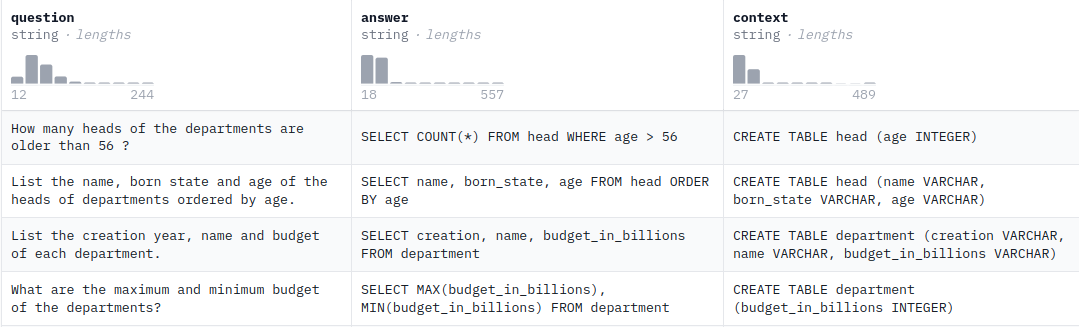
\includegraphics[width=14cm]{./data_head.png}
    \caption{Một vài dòng dữ liệu fine-tune trên custom dataset.}
\end{minipage}

\vspace{0.5cm}
Tiếp theo ta sẽ chỉ ra cách tokenize dữ liệu về dạng vector để đưa vào mô hình:
\begin{itemize}
    \item Đầu tiên, ta sẽ thêm vào một prefix là 'query for: ' để đánh dấu bắt đầu câu hỏi, thêm prefix là 'tables: ' để đánh dấu là ngữ cảnh.
    \item Với mỗi từ, xây dựng từ điển và đánh mỗi từ với 1 id riêng biệt
    \item Tokenize chuỗi đầu vào thành input-ids, thêm token '</s>' ở cuối để đánh dấu hết câu,
     thêm padding token để đảm bảo độ dài của input là như nhau (200 tokens).
    \item Tokenize chuỗi đầu đích thành decoder-input-ids, dịch tất cả các token sang phải, thêm start: token '<s>' ở đầu , 
    thêm token '</s>' ở cuối để đánh dấu hết câu, 
    thêm padding token để đảm bảo độ dài của input là như nhau (128 tokens).
    \item Khởi tạo attention mask, đánh dấu các token padding là 0, các token thật là 1.
\end{itemize}

Như vậy với các chuỗi là câu hỏi, ngữ cảnh và truy vấn SQL, ta đã có thể tokenize chúng thành các vector input-ids, decoder-input-ids, attention mask và decoder-attention-mask.

Ví dụ với chuỗi đầu vào là 

\textit{query for: what are the classes that having name start with 'A-' tables: CREATE TABLE classes (id INT, name TEXT); }, ta sẽ tokenize nó thành:


\vspace{0.2cm}
\begin{minipage}{\linewidth}
    \captionsetup{type=figure}
    \centering
    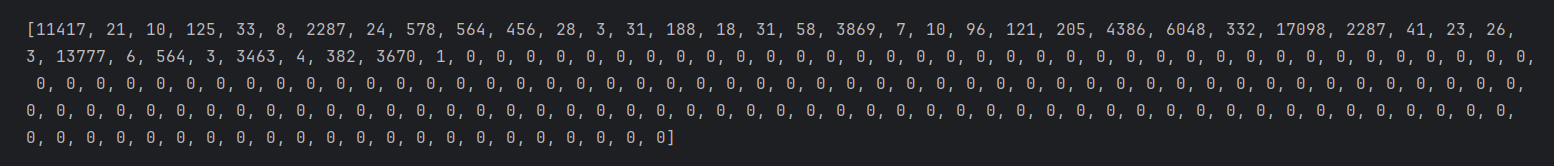
\includegraphics[width=14cm]{./input_ids.png}
    \caption{Tokenize chuỗi đầu vào.}
\end{minipage}

\vspace{0.5cm}
Xây dựng Dataloader và phân chia tập dữ liệu:
\begin{itemize}
    \item Tách tập dữ liệu thành 2 phần: 80\% train và 20\% test, trộn ngẫu nhiên các dòng cho hai tập
    \item Xây dựng lớp Dataloader, hỗ trợ quá trình train và test. Giúp lấy ra dòng dữ liệu theo index, trả về input-ids, decoder-input-ids, attention mask và decoder-attention-mask.
\end{itemize}

\subsection{Fine-tune mô hình}

\subsubsection{Thuật toán Lan Truyền Ngược (Backpropagation)}

Thuật toán lan truyền ngược là một thuật toán quan trọng trong học máy, được sử dụng để cập nhật các trọng số của mạng nơ-ron nhân tạo.
Thuật toán này sẽ tính toán đạo hàm của hàm lỗi (L) theo từng trọng số (w): 

Giả sử \( L \) là hàm lỗi (loss function) và \( w_i \) là trọng số thứ \( i \) trong mô hình. Đạo hàm của hàm lỗi theo \( w_i \) được ký hiệu là \( \frac{\partial L}{\partial w_i} \).

Thuật toán Lan Truyền Ngược (Backpropagation) được sử dụng kết hợp với
một thuật toán tối ưu hóa như Gradient Descent để cập nhật các trọng số.

Trong quá trình huấn luyện mô hình sử dụng thuật toán lan truyền ngược, ta cần 
thực hiện 3 bước sau để tính được đạo hàm của hàm lỗi theo từng trọng số:
\begin{itemize}
    \item Forward Pass: Tính toán giá trị của hàm lỗi (L) dựa trên các trọng số (w) hiện tại.
    \item Compute Local Gradients: Tính giá trị đạo hàm tại mỗi nút (node) trong mạng nơ-ron.
    \item Backward Pass: Tính toán đạo hàm của hàm lỗi (L) theo từng trọng số (w) hiện tại.
\end{itemize}

\begin{minipage}{\linewidth}
    \captionsetup{type=figure}
    \centering
    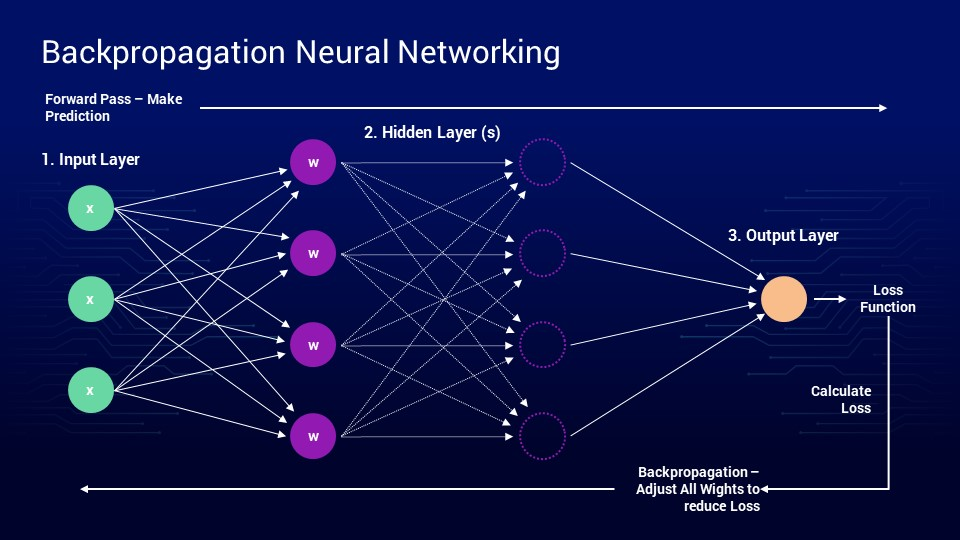
\includegraphics[width=12cm]{./back-propagation.jpg}
    \caption{Sơ đồ thuật toán Backpropagation. Nguồn ảnh: \textbf{SideSalad.com}}
\end{minipage}

Ở bước cuối cùng, sau khi có được giá trị hàm lỗi và đạo hàm tại mỗi nút mạng, ta tiến hành tính đạo hàm của hàm lỗi theo từng trọng số (w) hiện tại.
Kết hợp với \textit{Chain Rule} có quy tắc như sau:
Giả sử $f(x)$ và $g(x)$ là hai hàm có đạo hàm. Quy tắc chuỗi cho biết rằng đạo hàm của hàm hợp $h(x) = f(g(x))$ được tính theo công thức:

\[
(h \circ g)'(x) = f'(g(x)) \cdot g'(x)
\]

Trong ký hiệu toán học:

\[
\frac{d}{dx}[f(g(x))] = f'(g(x)) \cdot g'(x)
\]
\subsubsection{Gradient Descent - AdamW} 



\subsubsection{Hàm lỗi CrossEntropyLoss} 

\subsubsection{Fine-tune}
Do thiếu tài nguyên tính toán, nên việc huấn luyện cho mô hình chỉ được giữ ở mức tối thiểu. Các tham
số được lựa chọn để fine-tune lại mô hình như sau:

\begin{itemize}
    \item \textbf{Epoch}: 2
    \item \textbf{Batch size}: 16
    \item \textbf{Learning rate}: 3e-5
    \item \textbf{Optimizer}: AdamW
    \item \textbf{Loss function}: CrossEntropyLoss
\end{itemize}



Hai biểu đồ thể hiện giá trị lỗi trên tập train và tập test của mô hình:
\vspace{0.5cm}

\begin{minipage}{\linewidth}
    \captionsetup{type=figure}
    \centering
    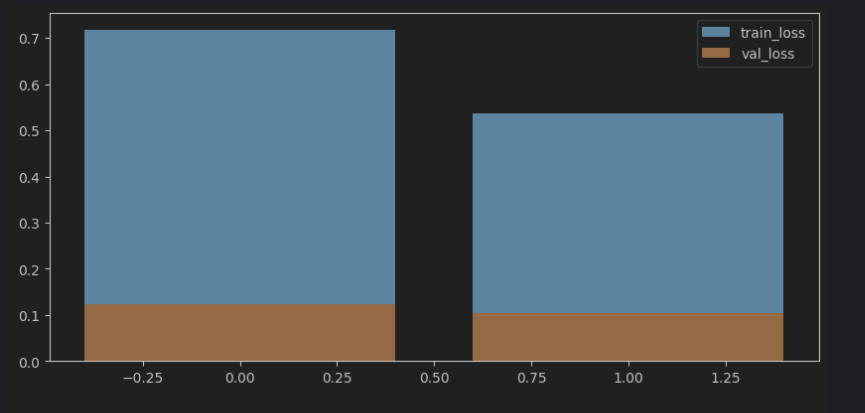
\includegraphics[width=10cm]{./bar_plot.png}
    \caption{Biểu đồ giá trị lỗi (cột) trên tập train và tập test.}
\end{minipage}

\begin{minipage}{\linewidth}
    \captionsetup{type=figure}
    \centering
    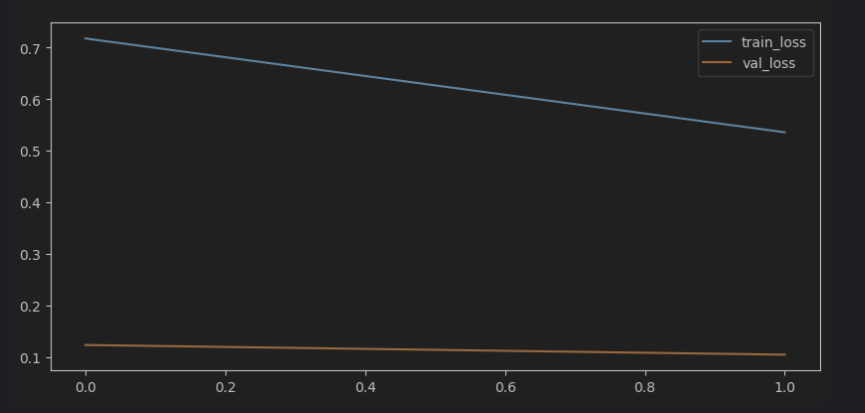
\includegraphics[width=10cm]{./plot.png}
    \caption{Biểu đồ giá trị lỗi (đường) trên tập train và tập test.}
\end{minipage}

\subsection{Đánh giá mô hình}

\section{Triển khai mô hình}

\newpage
\printbibliography

\end{document} % This is the end of the document